\documentclass[11pt]{article}
\usepackage[margin =1in]{geometry}
\usepackage{authblk}
\usepackage{lipsum}
\usepackage{multicol}
\usepackage{graphicx}
\usepackage{float}
\usepackage[hidelinks]{hyperref}
\usepackage{amsmath}
\usepackage[backend = bibtex, style = numeric, sorting = ynt]{biblatex}
\addbibresource{reference.bib}
\title{{\bf Computational Methods for RNA Secondary Structure Prediction}}
\author[1]{Harrison LaBollita}
\author[2]{Petr \u Sulc}
\date{}
\affil[1]{Department of Physics, Arizona State University, Tempe, AZ 85281 USA}
\affil[2]{Center for Biological Physics, Arizona State University, Tempe, AZ 85281 USA}

\begin{document}
\maketitle
\begin{abstract}
\lipsum[1]
\end{abstract}
\tableofcontents
\section{Introduction}
\lipsum[2-4]
\lipsum[2-4]
\section{Convolutional Neural Network Predicts Secondary Structure}
\subsection{Data and Methods}
\begin{figure}[H]
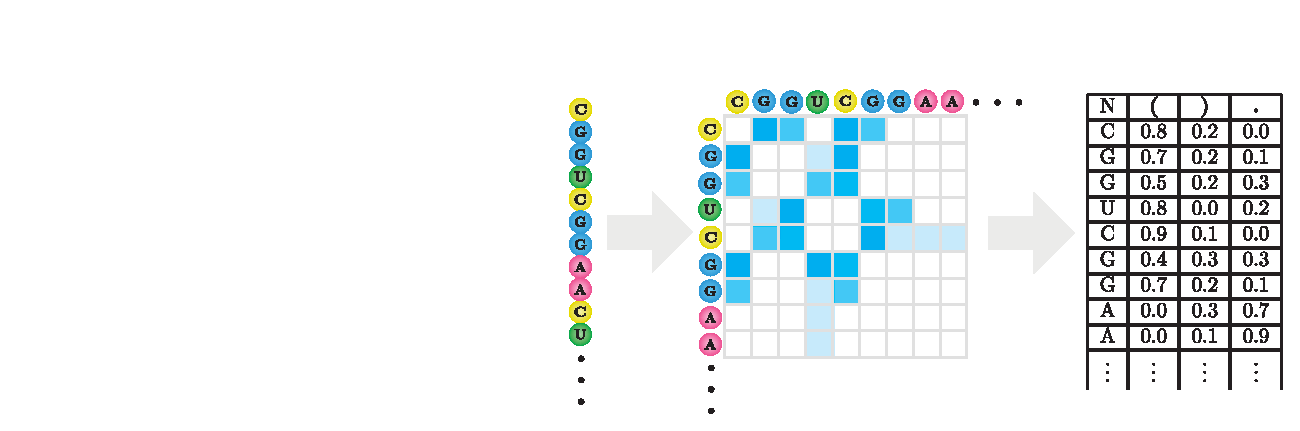
\includegraphics[width = \textwidth]{fig/cnn_model_outline}
\end{figure}
\lipsum[2]
\subsection{Convolutional Neural Network Model}
\lipsum[2]
\subsection{Results}
\lipsum[2]
\section{Stem Level Gillespie Algorithm}
\subsection{Introduction to Gillespie Algorithm}
\lipsum[1]
\subsection{Stem Level Implementation}

\begin{figure}[H]
\centering
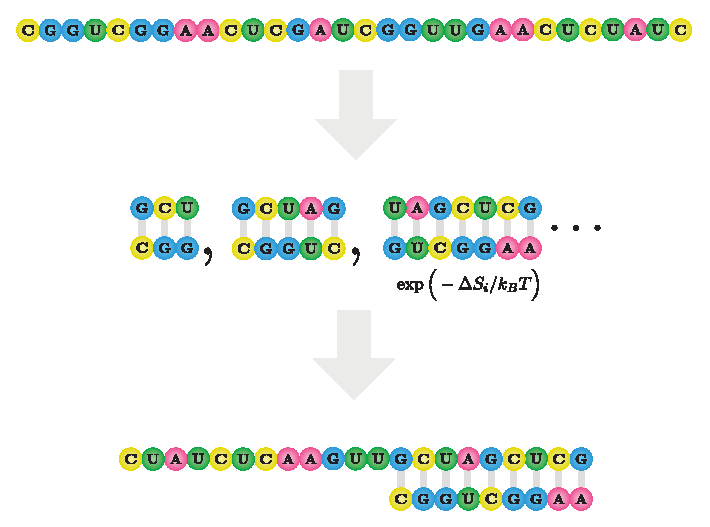
\includegraphics{fig/rna_gillespie_algo}
\end{figure}
\lipsum[2]
\subsection{Results}
\lipsum[2]
\section{Conclusion and Outlook}
\lipsum[2-4]
\lipsum[2-4]
\newpage
\nocite{*}
\printbibliography
\end{document}
